%\documentclass[9pt,twocolumn,twoside,lineno]{pnas-new}
\documentclass[9pt,twocolumn,twoside]{pnas-new}
% Use the lineno option to display guide line numbers if required.
\usepackage{graphicx}
\usepackage{textcomp}


\templatetype{pnasresearcharticle} % Choose template 
% {pnasresearcharticle} = Template for a two-column research article
% {pnasmathematics} %= Template for a one-column mathematics article
% {pnasinvited} %= Template for a PNAS invited submission

\title{Variation in recombination rate affects detection of $F_{ST}$ outliers under neutrality}
%Heterogeneous landscapes of average $F_{ST}$ arise under neutrality due to recombination rate variation}

% Use letters for affiliations, numbers to show equal authorship (if applicable) and to indicate the corresponding author
\author[a,b,1]{Tom R. Booker}
\author[c]{Samuel Yeaman} 
\author[b,d]{Michael C. Whitlock}

\affil[a]{Department of Forest and Conservation Sciences, University of British Columbia, Vancouver, Canada}
\affil[b]{Biodiversity Research Centre, University of British Columbia, Vancouver, Canada}
\affil[c]{Department of Biological Sciences, University of Calgary, Calgary, Canada}
\affil[d]{Department of Zoology, University of British Columbia, Vancouver, Canada}


% Please give the surname of the lead author for the running footer
\leadauthor{Booker} 


% Please include corresponding author, author contribution and author declaration information
\authorcontributions{Author contributions: T.R.B., S.Y., and M.C.W. designed research; T.R.B. performed research; and T.R.B., S.Y., and M.C.W. wrote the paper.}
\authordeclaration{The authors declare no competing interests}
\correspondingauthor{\textsuperscript{1}To whom correspondence should be addressed. E-mail: booker@zoology.ubc.ca}

% Keywords are not mandatory, but authors are strongly encouraged to provide them. If provided, please include two to five keywords, separated by the pipe symbol, e.g:

\keywords{Population structure $|$ Genome scan $|$ $F_{ST}$ $|$ Coalescence } 

\begin{abstract}
Genome scans can potentially identify genetic loci involved in evolutionary processes such as local adaptation and gene flow. Here, we show that recombination rate variation across a neutrally evolving genome gives rise to different sampling distributions of mean ${F_{ST}}$ (${\hat{F_{ST}}}$), a common population genetic summary statistic. In particular, we show that in low recombination regions the distribution of $\hat{F_{ST}}$ estimates may have a longer tail than in more highly recombining regions. Determining outliers from the genome-wide distribution without accounting for local recombination rate may therefore increase the frequency of false positives in low recombination regions and be overly conservative in more highly recombining ones. We perform genome-scans on simulated and empirical \textit{Drosophila melanogaster} datasets and, in both cases, find patterns consistent with this neutral model. Our results highlight a flaw in the design of genome scan studies and suggest that without estimates of local recombination rate, it is very difficult to interpret the genomic landscape of population genetic summary statistics.

\end{abstract}


\begin{document}

\maketitle
\thispagestyle{firststyle}
\ifthenelse{\boolean{shortarticle}}{\ifthenelse{\boolean{singlecolumn}}{\abscontentformatted}{\abscontent}}{}


Genome scans have become a standard analysis in population genetics used to identify genomic regions involved in important evolutionary processes. With a reference genome and DNA re-sequencing data, the genome can be divided into analysis windows of a fixed physical size and the distribution of summary statistics across those windows can be examined. Outliers to the genome-wide distribution of a particular summary statistic may then be investigated for their roles in processes such as adaptation and speciation. 

A particularly important summary statistic used in genome scans is Wright's $F_{ST}$. Wright \citep{RN200} examined the behaviour of allele frequencies in metapopulations and referred to the correlation of frequencies among demes as $F_{ST}$. The evolutionary history of a population can be thought of as a series of genealogies describing the relationships between every individual at a certain point in the genome, and Slatkin \citep{Slatkin1991} showed that for a neutrally evolving metapopulation $F_{ST}$ can be expressed in terms of the coalescence times of those genealogies. In particular, \begin{math} F_{ST} = \frac{\bar{T} - \bar{T_0}}{\bar{T}} \end{math}, where $\bar{T_0}$ is the average coalescence times for a pair of alleles drawn from the same deme and $\bar{T}$ is the average coalescence time for a pair of alleles drawn from the metapopulation as a whole. $F_{ST}$ varies across the genome; the mutations that happened to occur in the population and the individuals that happened to be sampled will give rise to variation in $F_{ST}$ at different points in the genome. There are numerous methods to average across linked sites in an attempt to account for these sources of variation (reviewed in \citep{Holsinger2009}). Furthermore, the underlying demographic process is also stochastic and will generate different histories across the genome generating heterogeneity in $F_{ST}$.  

In the context of genome scans, $\hat{F_{ST}}$ is calculated in analysis windows, and the genome-wide distribution is examined under the implicit assumption that all windows share the same sampling distribution. However, recombination breaks down associations across genetically linked sites allowing coalescence times to vary across the genome causing some windows to reflect more or fewer coalescent histories than others. Thus, the sampling distributions of summary statistics that capture aspects of coalescent history likely covary with the rate of recombination.

Consider a 10,000bp analysis window in a neutrally evolving genomic region that experiences virtually no recombination (for example, the mitochondrial genome or non-pseudoautosomal regions of the Y-chromosome in humans). Every nucleotide within this window would share a single genealogy, and every polymorphism present would reflect the exact same coalescent history. If there were a large number of polymorphisms in the window, the combined $\hat{F_{ST}}$ across all of them may provide a very precise estimate of their shared history. If one had a large number of these analysis windows and examined the distribution of their averages, it should resemble the coalescent distribution of $F_{ST}$, which, for a population conforming to the island model, can be approximated using the $\chi^2$ distribution \citep{Lewontin1973-uf}, which has a long upper tail.

Now consider the alternate extreme, 10,000bp of freely recombining nucleotides. In this case, all sites would have a distinct evolutionary history, each representing a quasi-independent instantiation of the coalescent process. As a result, every polymorphism in the window would carry information on a different genealogy, and each of these may have a distinct $F_{ST}$. The observed $\hat{F_{ST}}$ across all polymorphisms in this set provides an estimate of the mean of the coalescent distribution of $F_{ST}$. If one had a large number of these sets of loci, the values of $\hat{F_{ST}}$ should be tightly distributed about the mean, and central limit theorem predicts that the distribution should be approximately Gaussian. 

%\begin{figure}%[tbhp]
%\centering
%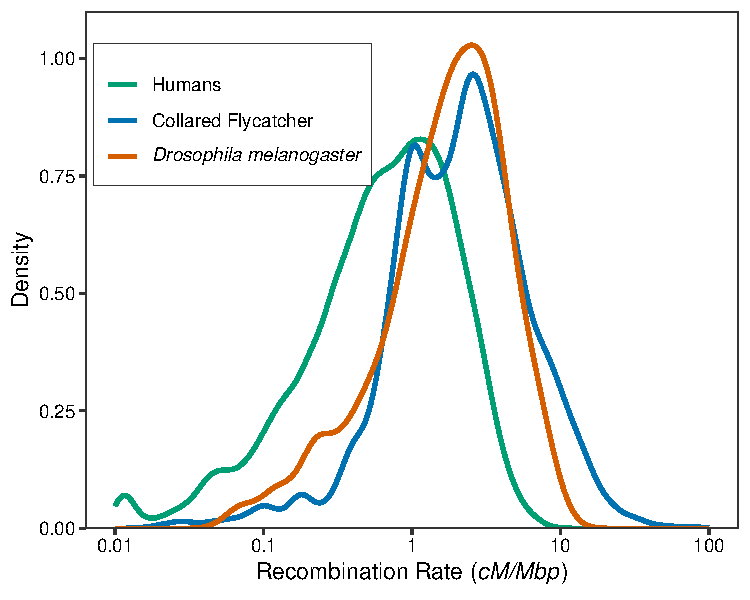
\includegraphics[width=.8\linewidth]{RecRateVariation.pdf}
%\caption{The distribution of recombination rates in three eukayotic species. Sex-averaged estiamtes of recombination rate for 200 Kbp regions are shown.}%\label{fig:recombination}
%\end{figure}

Obviously 10,000 contiguous nucleotides do not experience free recombination, but eukaryotes do exhibit wide variation in recombination rates across their genomes. For example, humans \cite{Kong2010}, collared flycatchers \cite{Kawakami2014} and \textit{Drosophila melanogaster} \citep{Comeron2012} all exhibit recombination rate variation over at least an order of magnitude across substantial proportions of their genomes. If the sampling distribution of $\hat{F_{ST}}$ had a longer tail in regions of the genome with low recombination and was narrower in more highly recombining ones, heterogeneous landscapes of $F_{ST}$ may arise under neutrality. Determining outliers from the genome-wide distribution of summary statistics may, therefore, result in false positives and negatives depending on the local recombination rate. In this study, we demonstrate that the sampling distribution of $\hat{F_{ST}}$ does indeed depend on the local recombination rate and show how this may affect genome-scans using simulated and empirical datasets.


%In particular we suggest that in low recombination cases, windows have more uniform genealogies and therefore more uniform values of observed $F_{ST}$, so that the few windows that by chance have extreme genealogies (in terms of among-populations differentiation) also have more extreme values of $F_{ST}$, on both ends of the spectrum. By contrast, the high recombination windows have more heterogeneity in their genealogies, such that even areas of the genome that chance to have extreme genealogies in terms of divergence among populations have less extreme values of $F_{ST}$.





\section*{Results and Discussion}
 
To determine whether the sampling distribution of $\hat{F_{ST}}$ is affected when recombination rates vary over orders of magnitude, we simulated genomic data under an island model of population structure. Different distributions of mean $\hat{F_{ST}}$ arose under different recombination rates (Fig. \ref{fig:Fst}). The theoretical expectation of $F_{ST}$ was the same in all of the simulations shown in Figure \ref{fig:Fst}, and the average $\hat{F_{ST}}$ was very close to the expectation in all cases. However, low recombination rates led to longer-tailed distributions of $\hat{F_{ST}}$ and higher rates led to distributions that were tighter about the mean (Fig \ref{fig:Fst}). 

A typical method for determining outliers in genome scans is to examine the top $n^{th}$ percentile of a particular summary statistic. If one were performing a genome scan in a species that exhibited recombination rate variation even over a single order of magnitude, one would expect the tail of the genome-wide distribution of $\hat{F_{ST}}$ to be enriched for analysis windows in low recombination regions under neutrality (Fig. \ref{fig:Fst}). Indeed, the recombination rates shown in Figure \ref{fig:Fst} obviously lead to different distributions of $\hat{F_{ST}}$, but the extent to which this will affect the analysis of real organisms will depend on the pattern of variation in recombination rates across their genomes.

\begin{figure}%[tbhp]
\centering
\includegraphics[width=.8\linewidth]{Fst_plot.pdf}
\caption{The distribution of $F_{ST}$ calculated in 10 Kbp windows. $F_{ST}$ was averaged using the method of Weir and Cockerham. The dashed vertical line is the theoretical expectation of $F_{ST}$ for the simulated population and the coloured vertical lines indicate the means for each set of simulations. }\label{fig:bottom}
\label{fig:Fst}
\end{figure}

%We compared the relationship between $F_{ST}$ and recombination rate in simulated populations with an empirical dataset from North American populations of \textit{Drosophila melanogaster} generated by Reinhardt et al \citep{Reinhardt2014-xq}.

We examined the relationship between $\hat{F_{ST}}$ and recombination rate across the \textit{D. melanogaster} genome using simulated and empirical datasets. We simulated the entire \textit{D. melanogaster} genome under a model of isolation-with-migration incorporating recombination rate variation using \textit{stdpopsim} \cite{adrion2019community} and performed genome scans on the resulting data (Fig. \ref{fig:drosophila}). We performed a similar genome scan on the population genomic data from North American \textit{D. melanogaster} populations generated by Reinhardt et al \cite{Reinhardt2014-xq}. In both cases, we found a significant enrichment of outliers at low recombination rates compared to high recombination rates when we defined outliers based on the $95^{th}$ percentile of $\hat{F_{ST}}$ 
(simulated data Fisher's exact test \textit{p-value} < $10^{-15}$; empirical data Fisher's exact test \textit{p-value} = 0.00265). Furthermore, both the simulated and empirical datasets exhibited significant negative correlations between the variance of $\hat{F_{ST}}$ and recombination rate (Fig. \ref{fig:drosophila}C; simulated data, Kendall's $\tau$ = -0.746, \textit{p-value} < $10^{-15}$; empirical data, Kendall's $\tau$ = -0.193, \textit{p-value} = $0.00445$). Of course, the genomic landscape of $\hat{F_{ST}}$ in North American \textit{D. melanogaster} has likely been shaped by processes other than just migration and genetic drift. Indeed, Figure \ref{fig:drosophila}B shows at least one $\hat{F_{ST}}$ outlier at high recombination rates, which our simulations suggest would be unlikely under neutrality (Fig. \ref{fig:drosophila}A). In summary, our findings suggest that applying fixed thresholds to the genome-wide distribution of $\hat{F_{ST}}$ may enrich for false positives in low recombination regions and be overly conservative in highly recombining regions of the genome. 

%However, our simulations suggest that high $F_{ST}$ should not be uncommon in ow recombination rate regions, so perhaps $F_{ST}$ outliers in highly recombining regions should be 

%aberrantly 
%Since the $F_{ST}$ outlier 

%the highlighted $\hat{F_{ST}}$ outlier found in highly recombining regions, but the values  


%From Figure \ref{fig:drosophila}A it is obvious that defining outliers with a single cut-off would result in a large number of false positives. On the other hand, the empirical data shown in Figure \ref{fig:drosophila}B suggests that applying a single significance threshold might be conservative. 

% However, we do expect between the variance of $\hat{F_{ST}}$ and recombination rate in both the simulated and the empirical datasets.
%the simulated and the empirical \textit{D. melanogaster} data exhibited a negative relation


%The simulations we performed were strictly neutral and the means of the distributions shown in Figure \ref{fig:Fst} were almost identical, so we do not expect a significant correlation between recombination rate and $\hat{F_{ST}}$. However, we do predict a negative correlation between the variance of $\hat{F_{ST}}$ and the local recombination rate. 
 
%The recombination rates shown in Figure 2 obviously lead to different distributions of mean $F_{ST}$. The means of each of the distributions shown are very close to the theoretical expectation, which suggests that recombination rate variation alone would not generate a correlation between $F_{ST}$ and local recombination rate. However, we do predict a negative correlation between the variance of $F_{ST}$ and the local recombination rate.


%We tested that prediction by examining the distribution of $F_{ST}$ across the \textit{Drosophila melanogaster} genome using data from Reinhardt et al \citep{Reinhardt2014-xq}. In that study, the authors performed $F_{ST}$ genome scans on \textit{D. melanogaster} populations from North America. Fig \ref{fig:drosophila} shows the scatter plot of $\hat{F_{ST}}$ calculated in 10 Kbp windows against local recombination rate for the North American population of \textit{D. melanogaster} collected by Reinhardt et al \citep{Reinhardt2014-xq}. Genome-wide, there is a non-significant, weak correlation between $\hat{F_{ST}}$ and local recombination rate (Kendall's $\tau$ = -0.002; \textit{p-value} = 0.802). On the other hand, there was a strong, significant negative correlation between the variance of $F_{ST}$ and recombination rate, consistent with a neutral model with recombination rate variation (Kendall's $\tau$ = -0.302; \textit{p-value} < $10^{-10}$). Of course, the genomic landscape of $\hat{F_{ST}}$ in \textit{D. melanogaster} has likely been shaped by processes other than just migration and genetic drift. However, our results suggest that heterogeneous landscapes of $\hat{F_{ST}}$ can arise due to recombination rate variation in neutral models, and this should be incorporated into interpretation of genome scans. 

The effects of selection at linked sites, particularly background selection, have been invoked to explain patterns of variation in $F_{ST}$ across the genome \cite{Cruickshank2014-ps,Burri2017-ay}. Linked selection is most effective when recombination rates are low, so may cause heterogeneity in $F_{ST}$ across the genome. Closely related species that have correlated recombination rate landscapes and syntenic genomes may experience similar background selection effects and thus exhibit similar variation in $\hat{F_{ST}}$ \cite{Burri2017-ay}. However, recent work has shown that background selection may have quite limited effects on $F_{ST}$ in many cases \cite{matthey2019background}, so other explanations are perhaps required to explain genome-wide variation in $\hat{F_{ST}}$. Notably, species with correlated recombination landscapes may be prone to exhibiting high $F_{ST}$ in similar regions. Under neutrality, $\hat{F_{ST}}$ does not systematically vary as a function of recombination rate, but the potential to be an outlier does. Overlapping $F_{ST}$ outliers may then be mistaken for convergent adaptive evolution. 

We have focussed on $F_{ST}$ in this study, but it has long been known that the variance of summary statistics such as the number of segregating sites responds to variation in recombination rate \cite{Wakeley2009}, so the  difficulty of comparing analysis windows of discrete physical size across varying recombination rates likely extends to other data summaries as well. For example, absolute nucleotide diversity between populations ($D_{XY}$) is often used in conjunction with $F_{ST}$ in genome scans. We calculated $D_{XY}$ from our simulated data and found that the variance of that statistic was also negatively correlated with recombination rate (\textit{data not shown}). 

The results from this study should emphasise the need to incorporate recombination into the null model used to interpret genome scans. Without estimates of the local recombination rate it will be difficult to determine whether a particular statistical outlier is driven by adaptive or neutral processes. 


\begin{figure*}[\sidecaptionrelwidth]
\centering
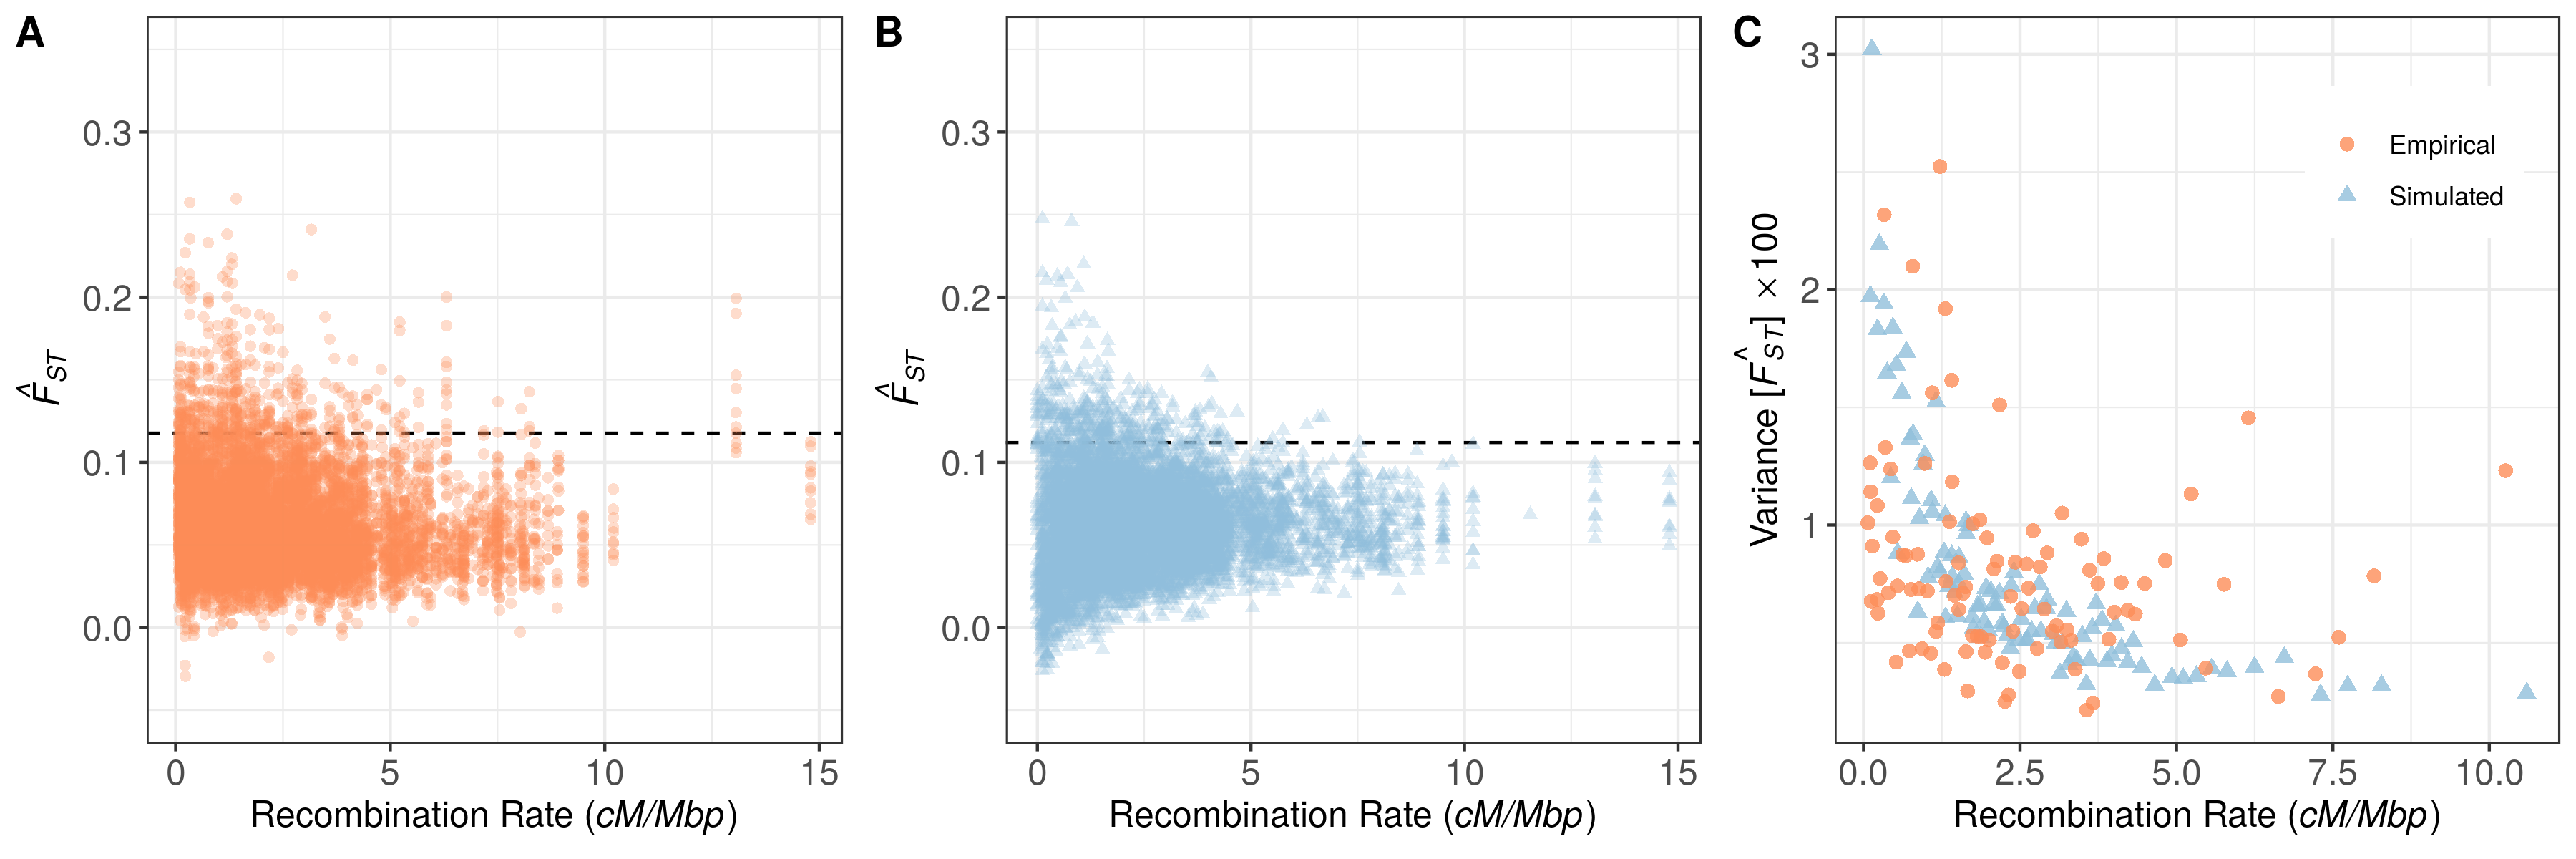
\includegraphics[width=\linewidth]{threePanelFigure.png}
\caption{The plot of $\hat{F_{ST}}$ calculated in 10,000bp analysis windowsd against local recombination rate for \textit{Drosophila melanogaster} from  A) the North American populations of \textit{Drosophila melanogaster} analysed by Reinhardt et al \cite{Reinhardt2014-xq} and B) coalescent simulations of the genome under a model of isolation with migration. C) Shows the variance in $\hat{F_{ST}}$ against recombination rate for both empirical and simulated datasets. The horizontal lines are the 95th percentiles of the genome-wide distribution in each case}\label{fig:drosophila}
\end{figure*}



\section*{Methods}

Coalescent simulations of structured populations were performed using \emph{msprime} v0.7.3 \cite{Kelleher2016-zz}. We simulated an island model of 100 demes, each with $N_e$ = 100 haploid individuals. Migration was constant between all demes and was set to $M$ = $N_em$ = 2, giving an expected $F_{ST}$ of $0.1\dot{1}$. After simulating a particular population, we added mutations to the resulting tree sequence at a rate of $10^{-6}$ then sampled 10 diploid individuals each from two demes and calculated the weighted average of $F_{ST}$ using the method for diploids given in Weir \cite{weir1990genetic} as implemented in \emph{scikit-allel} v1.2.1. We repeated this procedure 100 times for each simulated population and took the average across replicates. We performed 1,000 such simulations for each recombination rate tested.

We analysed allele frequency data from the North American \textit{Drosophila} populations analysed by Reinhardt et al \citep{Reinhardt2014-xq}. In that study, pooled sequencing was used to estimate derived allele frequencies for pools of 16 isofemale lines each from Maine and Florida. To obtain accurate allele freuqencies we excluded any single nucleotide polymorphism that was reported at a depth greater than or less than one standard deviation from the mean coverage. 

We simulated the entire \textit{Drosophila melanogaster} genome under a model of isolation with migration model in \textit{stdpopsim} v0.1.1. An ancestral population with effective size $2N_e = 344,120$ individuals, split into two demes of $N_e$ individuals $N_e$ generations in the past. Symmetrical migration of $m = \frac{3}{2N_e}$ migrants per generation occurred after the split. The migration rate was chosen match $F_{ST}$ with the empirical data. We sampled 20 haploid individuals from each deme.

We analysed the genome-wide distribution of $F_{ST}$ in the empirical and simulated \textit{Drosophila melanogaster} datasets. Because the Reinhardt et al \citep{Reinhardt2014-xq} data was generated using pooled-sequencing, we calculated $F_{ST}$ for each polymorphism and averaged across sites using the formulae for haploids given in Weir \cite{weir1990genetic}. $\hat{F_{ST}}$ was calculated in 10,000bp non-overlapping windows using the ratio-of-averages approach. Recombination rates were extracted from the Comeron et al \cite{Comeron2012} map. For both the simulated and empirical \textit{D. melanogaster} data, we examined the relationship between the variance of $\hat{F_{ST}}$ and recombination rate by dividing the recombining genome into 75 equally sized bins. We calculated Kendall's correlation between the variance of $\hat{F_{ST}}$ and the mean recombination rate in these bins. We classified analysis windows as outliers if $\hat{F_{ST}}$ was greater than the $95^{th}$ percentile genome-wide. We examined the analysis windows with the 1,000 largest and smallest recombination rate estimates and used Fisher's exact test to determine whether there was a significant enrichment of outliers in low recombination regions. We excluded analysis windows from the simulated data that had recombination rates of 0.

\subsection*{Data availability} Python scripts implementing the simulations shown as well as additional population models are available at \url{https://github.com/TBooker/Recombination_Fst}.

\acknow{Thanks to Sally Otto, Andr\'ea Thomaz and Wouter van der Bijl for helpful discussions and to Matt Pennell for comments on the manuscript. Thanks to Andrew Kern for insights and for providing the \textit{Drosophila} data. This project is part of the CoAdapTree project which is funded by Genome Canada (241REF), Genome BC and 16 other sponsors (\url{http://coadaptree.forestry.ubc.ca/sponsors/}). MCW is supported by a Discovery Award from NSERC. SY is supported by a Discovery Award from NSERC and a research chair from Alberta Innovates.}

\showacknow{} % Display the acknowledgments section

% Bibliography
\subsection*{References}
\bibliography{VariableRecomReferences}

\end{document}



I downloaded the human recombination maps from Kong et al (2010) from http://www.decode.com/addendum.

Kong
Comeron
Kawakami
Slatkin
Weir and Holsinger
Weir and Cockerham
Fst_review
Wright 1937
Lewontin and Krakauer
Kelleher
sci-kit


